\section{DynamoDB - Zhaoheng Wang}
	\subsection{Data structure organization}
     In general, the project will start with parsing sample data from s3. After that, the sample data will be processed and store into the DynamoDB. Finally,  we will do the analysis in the QuickSight based on the sample data. Before loading data into DynamoDB, the table and the data structure should be organized. Therefore, the first job for me is to figure out the data structure before creating table. Unlike the relational database, the ER-diagram is not suitable for organizing data structure in DynamoDB. In the DynamoDB, we treat each rows of sample data as an individual item and each column will be the attribute for the item. When we load the data into table, we are loading the items into the table in DynamoDB. For instance, we need to store the wireless information for different users based on sample data such as connecting time, disconnecting time, information of device, average usage and operating system they use. In this case, we treat each user as individual items and the wireless information for that user will be the attributes. Based on the sample data, there will be three tables in the Dynamodb. The first table is the table which contains almost all the attributes except mac address and Onid. Instead, there will be two link tables which contains the mac address and Onid. Each table will have unique key pin and pin is actually Onid hash with some random strings.The figure \ref{fig:1} is showing the table structure on DynamoDB.
\begin{figure}[H]
 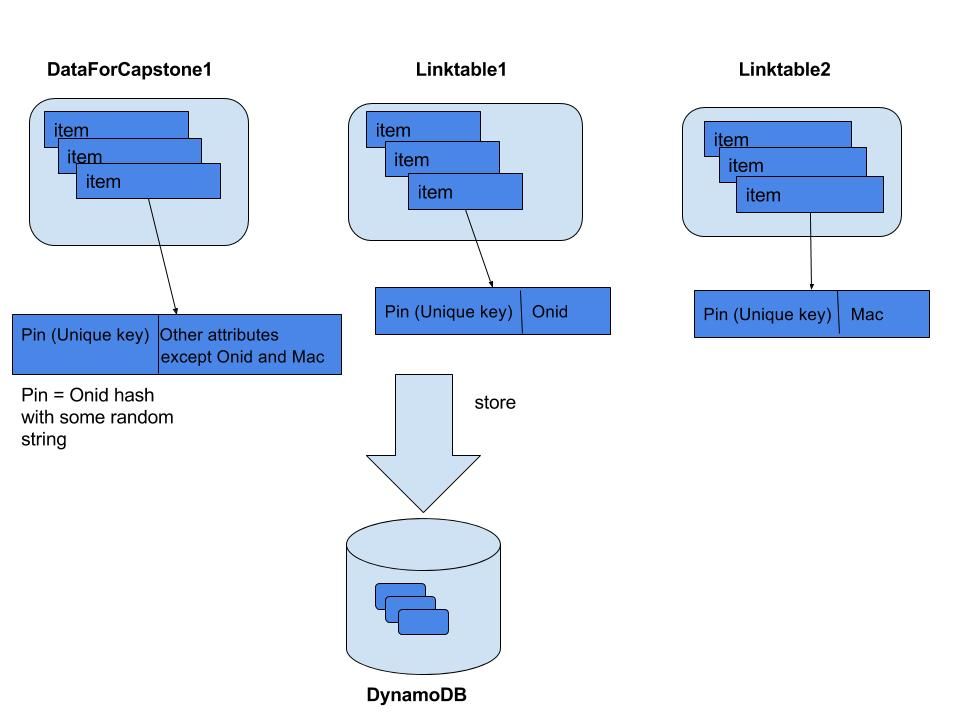
\includegraphics[width=17cm, height=7cm]{7.jpg}
 \centering
 \caption{\label{fig:1}Table structure}
 \end{figure}
 
 \subsection{Workflow of loading new data }
 	The workflow of loading new data into DynamoDB starts with S3. At first, the system stores the new record in S3. After that, it checks whether the identifier for the device or person is new. If the unique identifiers are new, a new system identifier is generated based on a hash of the original device and student identifiers. The original identifiers and the new identifier are then added to a restricted access, DynamoDB Identity table. In the record, the original identifiers are replaced with the new system identifier, and the anonymized record is loaded into a DynamoDB data table. If the unique identifiers are not new, they are replaced with the system identifier already available in the Identity table, and the record is added to the data table.The figure \ref{fig:2} is workflow of loading new data.
\begin{figure}[H]
 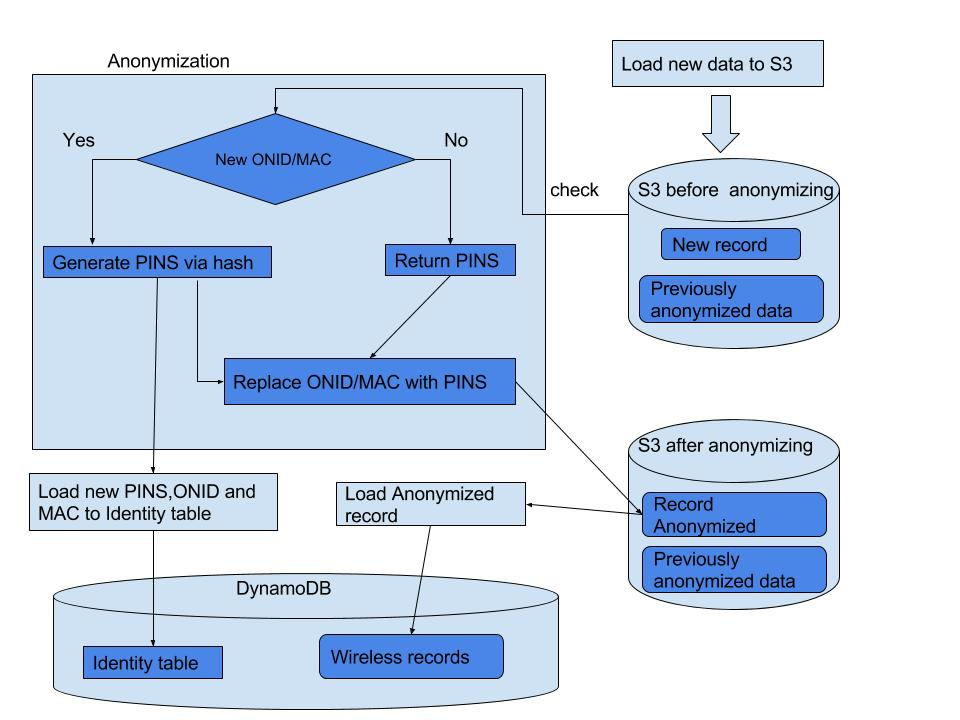
\includegraphics[width=17cm, height=8cm]{8.jpg}
 \centering
 \caption{\label{fig:2}The workflow of loading new data}
 \end{figure}